\chapter{RESULTS AND DISCUSSION}

A set of performance indicators is employed to assess the 
operational quality of a signalized intersection, with queue 
lengths, delays, vehicle travel time, and LOS being primary 
measures. These indicators are interrelated as output parameters.

\section{Queue length as a performance Indicator}

Queue lengths refer to the number of vehicles waiting behind 
the stop line during a red signal phase, and delays represent
 the time vehicles spend in the queue. Common indicators 
 include average queue length and average delays, expressed 
 numerically or as percentages. The queue length ratio is 
 calculated by dividing the average queue length ($q_i$) by its 
 maximum value ($Q_{max}$), as defined in Equation:

 \begin{equation*}
    Queue length ratio = \frac{1}{n} \sum_{i=1}^{n} \frac{q_i}{Q_{max}}
 \end{equation*}

 \subsection{Peak Hour Analysis}
The figure displays the queue length comparison across three 
scenarios for various traffic routes and intersections.

%figure
\begin{figure}[ht]
    \centering
    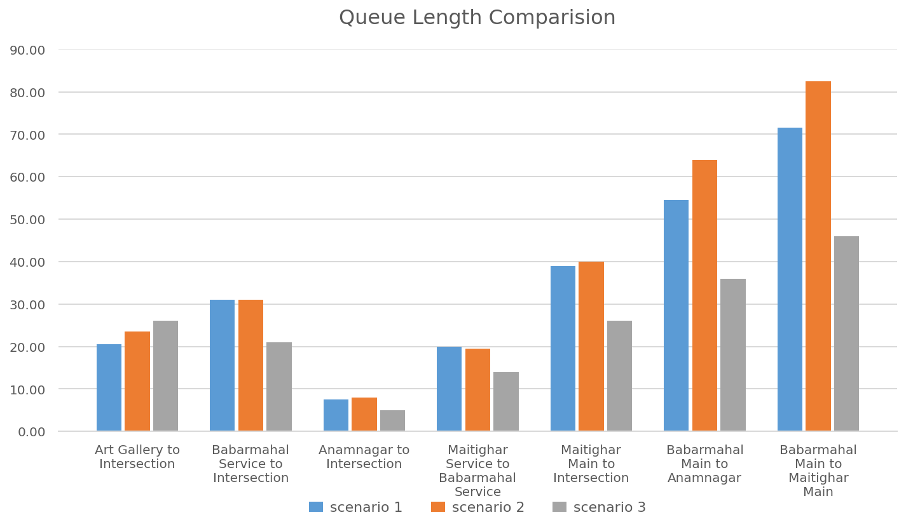
\includegraphics[width=\textwidth]{src/images/figures/1.png}
    \caption{Queue length - Peak Hour}
 \end{figure}


The peak hour queue length comparison reveals the same 
overarching trend observed during off-peak hours. Scenario 2 
either maintained or worsened queuing relative to the 
baseline, while Scenario 3 consistently delivered the lowest 
queue lengths across all movements. The Babarmahal Main to 
Maitighar Main movement dominates with the highest absolute 
values of 71.52 m, 82.87 m, and 46.00 m across Scenarios 1, 
2, and 3, respectively, where Scenario 2 worsened queuing by 
approximately 15.9 \% before Scenario 3 achieved a reduction 
of 35.7\% from the baseline. Babarmahal Main to Anamnagar 
follows closely with values of 54.86 m, 64.52 m, and 35.77 m, 
reflecting the same pattern of Scenario 2 amplifying the West 
approach queuing before Scenario 3 brought it under control 
with a 34.8\% reduction. The Maitighar Main to Intersection 
movement recorded values of 39.54 m, 40.26 m, and 26.43 m, 
with Scenario 3 reducing queue length by approximately 33.2\% 
from the baseline. For the lighter movements, Art Gallery to 
Intersection, Babarmahal Service to Intersection, Anamnagar 
to Intersection, and Maitighar Service to Babarmahal Service 
queue lengths remain comparatively low across all scenarios, 
yet Scenario 3 still achieves the lowest values in each case,
 confirming that even during off-peak conditions, the manually 
 optimized timing plan produces genuine and consistent 
 reductions in queue accumulation across all approaches of 
 the Babarmahal Intersection.


 \subsection{Off-Peak Hour Analysis}


 The table displays the queue length comparison across three 
 scenarios for various traffic routes and intersections.
%figure
\begin{figure}[ht]
    \centering
    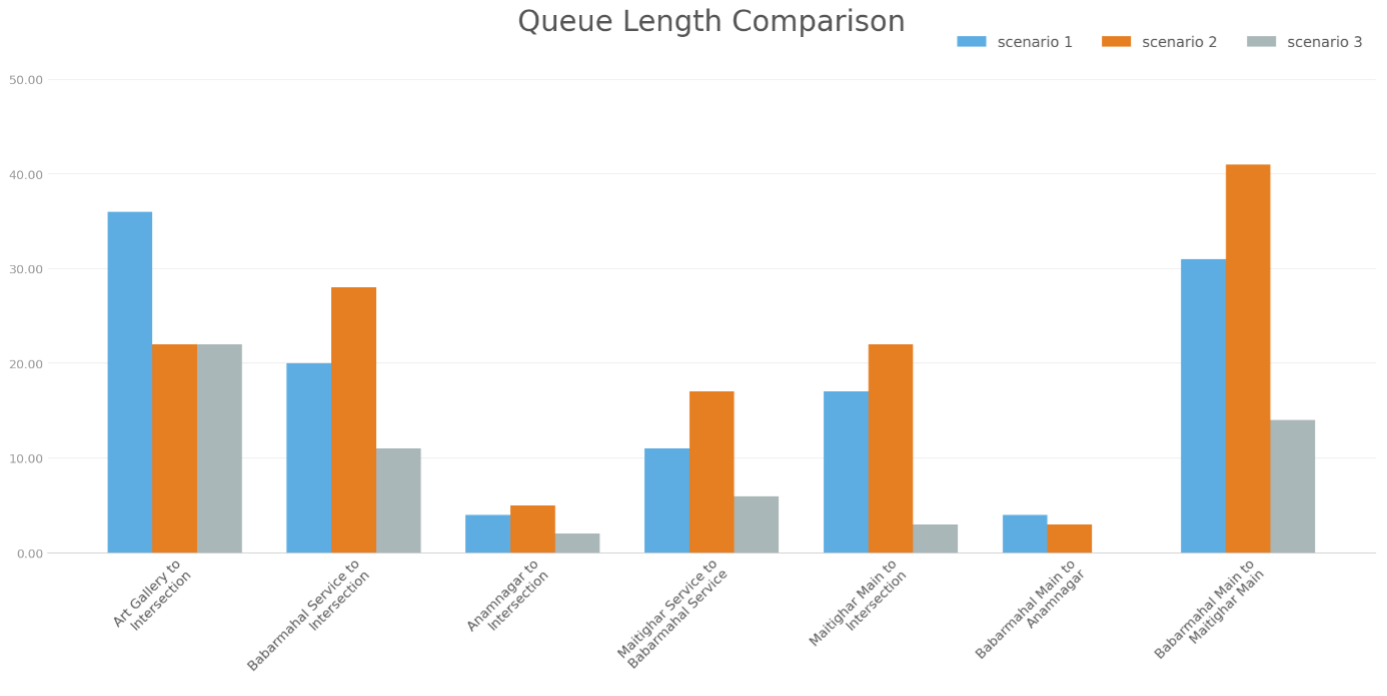
\includegraphics[width=\textwidth]{src/images/figures/2.png}
    \caption{Queue Length Off-Peak Hour}
 \end{figure}


The most telling indicator is the overall intersection queue 
length, which moves from 17.52 m (S1) -19.81 m (S2) -8.33 m 
(S3). This reveals that Scenario 2 actually worsened overall 
queue length compared to the baseline, while Scenario 3 
achieved a remarkable 52.5\% reduction from the baseline, 
the most significant system-wide improvement.

Maitighar Main to Intersection movement stands out as the 
most striking improvement across all scenarios. Starting at a 
queue length of 17.14 m in Scenario 1, it worsened to 22.11 m 
in Scenario 2, indicating that early interventions provided 
no relief for this approach. However, in Scenario 3, the 
queue length dropped dramatically to 2.72 m, a reduction of 
approximately 84\% from the baseline. 

 \section{Queue Delay as a Performance Indicator}

Delay refers to the amount of time spent passing through an 
intersection, the difference between arrival time and 
departure time, which can be determined in various ways. 
The vehicle delay ratio is calculated over the duration of 
the cycle length.

 \subsection{Peak Hour Analysis}

The figure displays the queue delay comparison across three 
scenarios for various traffic routes and intersections.
%figure
\begin{figure}[ht]
    \centering
    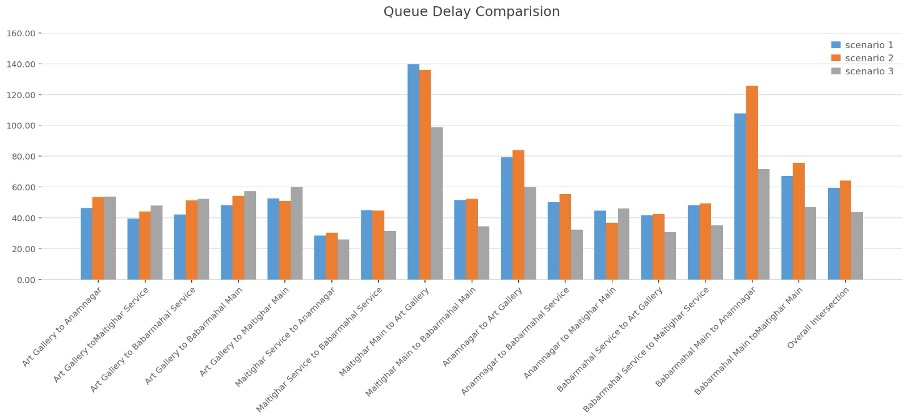
\includegraphics[width=\textwidth ]{src/images/figures/3.jpg}
    \caption{Queue Delay : Peak Hour}
 \end{figure}


The queue delay comparison across the three scenarios 
demonstrates a consistent and decisive improvement under 
Scenario 3 across nearly all movements at the Babarmahal 
Intersection. The overall intersection queue delay follows 
the trend of 60.26 sec/veh (Scenario 1) to 63.45 sec/veh 
(Scenario 2) to 44.82 sec/veh (Scenario 3), again confirming 
that Scenario 2 marginally worsened delay compared to the 
baseline, while Scenario 3 delivered a reduction of 
approximately 25.6\%; the most effective outcome overall. 
The most pronounced improvement is observed at the Maitighar 
Main to Art Gallery movement, which recorded the highest 
delays across all scenarios at 138.54, 132.18, and 97.23 
sec/veh, respectively, where Scenario 3 achieved a reduction 
of nearly 29.8\% from the baseline. Similarly, Babarmahal 
Main to Anamnagar exhibited notably high delays of 105.34 
sec/veh under Scenario 1, worsening to 124.67 sec/veh under 
Scenario 2, before Scenario 3 reduced it to 70.45 sec/veh: a 
reduction of approximately 33.1\%. For the remaining 
movements including Art Gallery to Anamnagar, Art Gallery 
to Maitighar Service, Art Gallery to Babarmahal Service, 
and Maitighar Service groups, delays remained in the 
moderate range of 40-60 sec/veh across all scenarios, with 
Scenario 3 consistently recording the lowest values, 
reinforcing that the manually optimized timing plan achieved 
broad and balanced delay reductions across the entire 
intersection rather than benefiting select movements in 
isolation.

 \subsection{Off-Peak Hour Analysis}

 The figure displays the queue delay comparison across three 
 scenarios for various traffic routes and intersections.

 %figure
 \begin{figure}[ht]
    \centering
    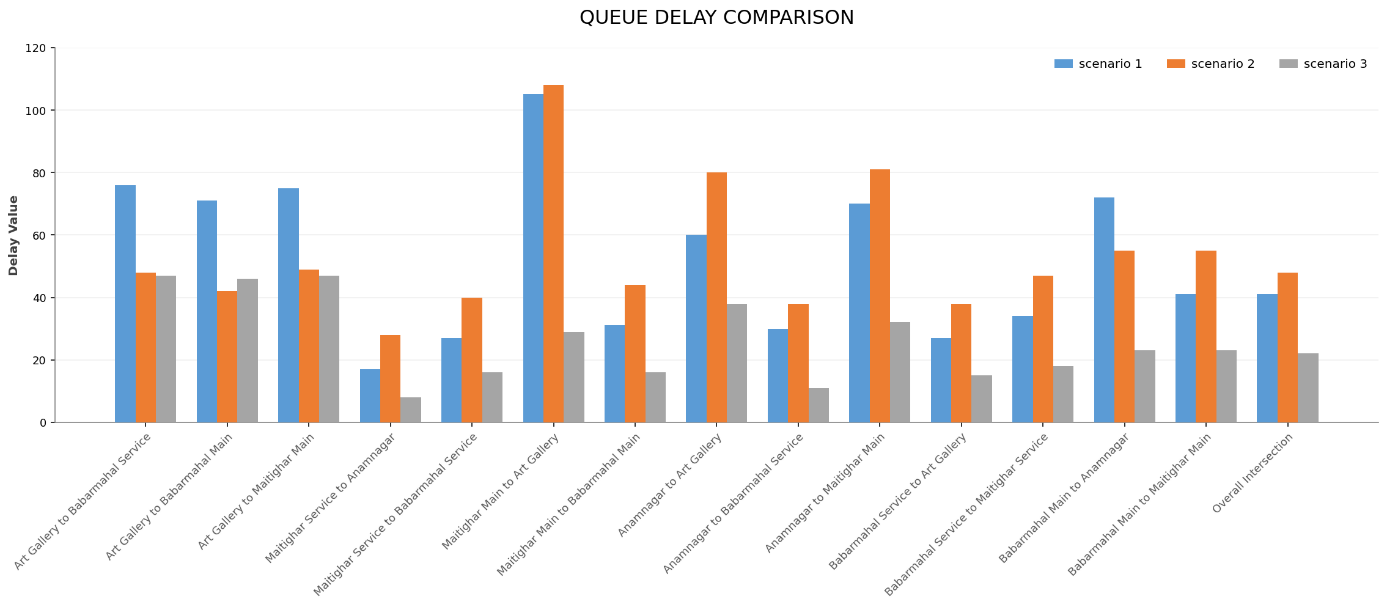
\includegraphics[width=\textwidth ]{src/images/figures/4.png}
    \caption{Queue Delay: Off-Peak Hour}
 \end{figure}


 The most telling indicator is the overall intersection queue 
 delay, which moves from 41.49 sec (S1) -48.83 sec (S2) -22.51 
 sec (S3). This reveals that Scenario 2 actually worsened 
 overall delay compared to the baseline, while Scenario 3 
 achieved a remarkable 45.7\% reduction from the baseline, 
 the most significant system-wide improvement.

 Maitighar main to Art Gallery movement stands out as one of 
 the most striking improvements across all scenarios. Starting 
 at a very high queue delay of 105.69 sec in Scenario 1, it 
 slightly worsened to 107.90 sec in Scenario 2, indicating 
 that early interventions provided no relief for this 
 approach. However, in Scenario 3, the delay dropped 
 dramatically to 29.68 sec, a reduction of approximately 72\% 
 from the baseline. 


 \section{Vehicle Travel Time}

 Vehicle travel time refers to the total time a vehicle 
 takes to traverse a defined road segment or network link 
 from one point to another, typically measured in seconds or 
 minutes. It encompasses both the free-flow travel time 
 under uncongested conditions and any additional delay 
 caused by traffic signals, congestion, turning movements, 
 or other impediments. It is a fundamental measure of traffic 
 performance, directly reflecting the efficiency and quality 
 of traffic flow along a corridor or intersection approach.


 \subsection{Peak Hour Analysis}

 The figure displays the vehicle travel time comparison across 
 three scenarios for various traffic routes and intersections.

 %figure
 \begin{figure}[ht]
    \centering
    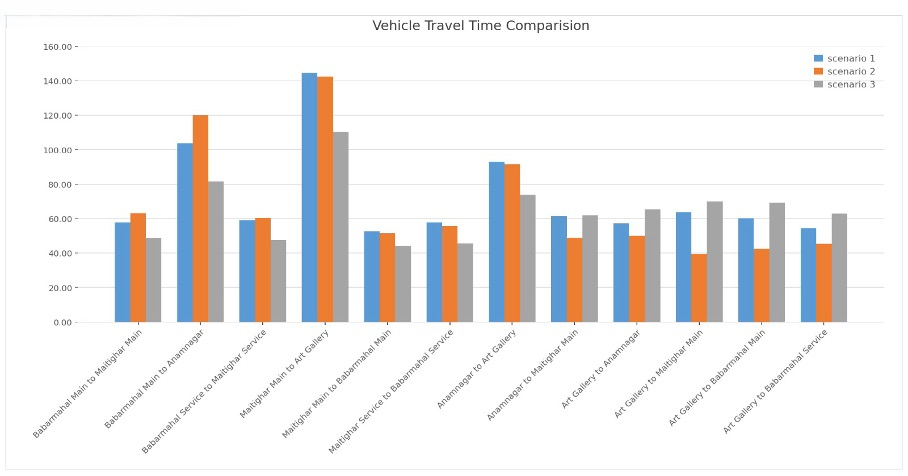
\includegraphics[width=\textwidth ]{src/images/figures/5.jpg}
    \caption{Vehicle Travel Time: Peak Hour}
 \end{figure}


 The vehicle travel time comparison across the three scenarios 
 presents a subtle picture, distinguishing it from the queue 
 delay and queue length results. The Maitighar Main to Art 
 Gallery movement records the highest travel times across 
 all scenarios at 143.25, 140.87, and 109.34 sec respectively, 
 with Scenario 3 achieving the most significant reduction of 
 approximately 23.7\% from the baseline. Babarmahal Main to 
 Anamnagar follows a similar pattern, rising from 103.45 sec 
 in Scenario 1 to 119.67 sec in Scenario 2 before dropping to 
 80.12 sec under Scenario 3 — a reduction of approximately 
 22.5\% — again highlighting that Scenario 2 worsened 
 conditions on the heavily loaded West approach before manual 
 optimization provided meaningful relief. Notably, for 
 several movements, including Art Gallery to Maitighar Main, 
 Art Gallery to Babarmahal Service, and Babarmahal Service to 
 Art Gallery, Scenario 2 actually recorded lower travel times 
 than both Scenario 1 and Scenario 3, suggesting that the 
 VISSIM-optimized timing selectively favored certain lighter 
 movements at the expense of the heavier ones. For the 
 remaining movements, travel times across all three scenarios 
 remain within a moderate range of 45-70 sec with marginal 
 differences, indicating that Scenario 3 delivers the most 
 balanced overall travel time distribution across the Babarmahal 
 Intersection without significantly penalizing any individual 
 movement.

 \subsection{Off-Peak Hour Analysis}

 The figure displays the vehicle travel time comparison 
 across three scenarios for various traffic routes and 
 intersections.

 %figure
 \begin{figure}[ht]
    \centering
    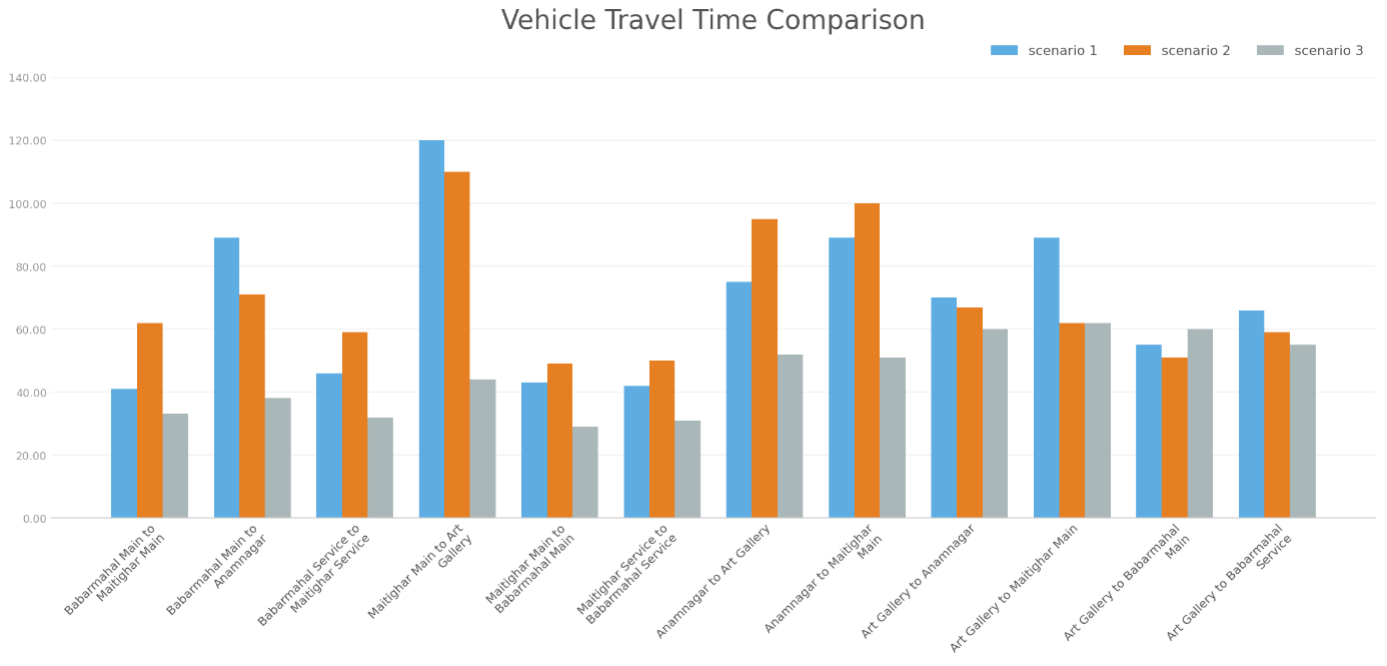
\includegraphics[width=\textwidth ]{src/images/figures/6.png}
    \caption{Vehicle Travel Time: Off-Peak Hour }
 \end{figure}


 The most telling indicator is the overall intersection 
 vehicle travel time, which moves from 68.87 sec (S1) → 
 69.49 sec (S2) → 45.81 sec (S3). This reveals that Scenario 
 2 actually worsened overall travel time compared to the 
 baseline, while Scenario 3 achieved a remarkable 33.5\% 
 reduction from the baseline, the most significant system-wide 
 improvement.

 Maitighar Main to Art Gallery movement stands out as the 
 most striking improvement across all scenarios. Starting at 
 the highest travel time of 120.34 sec in Scenario 1, it 
 partially improved to 109.79 sec in Scenario 2, indicating 
 that early interventions provided only marginal relief for 
 this approach. However, in Scenario 3, the travel time 
 dropped dramatically to 44.60 sec, a reduction of 
 approximately 63\% from the baseline. 


 \section{LOS}

 Level of Service (LOS) is a qualitative measure used to 
 characterize traffic flow conditions and the degree of 
 congestion experienced by road users. Defined by the 
 Highway Capacity Manual (HCM), LOS is graded on a scale 
 from A to F, where LOS A represents free-flow conditions 
 with minimal delay and LOS F denotes a complete breakdown 
 of traffic flow with excessive delays. For signalized 
 intersections, LOS is typically determined based on the 
 average control delay per vehicle (in seconds), serving as 
 a key indicator of operational performance and intersection 
 efficiency.


 \subsection{Peak Hour Analysis}

The figure displays the Level of Service (LOS) comparison across 
three scenarios for various traffic routes and intersections:

%figure
\begin{figure}[ht]
    \centering
    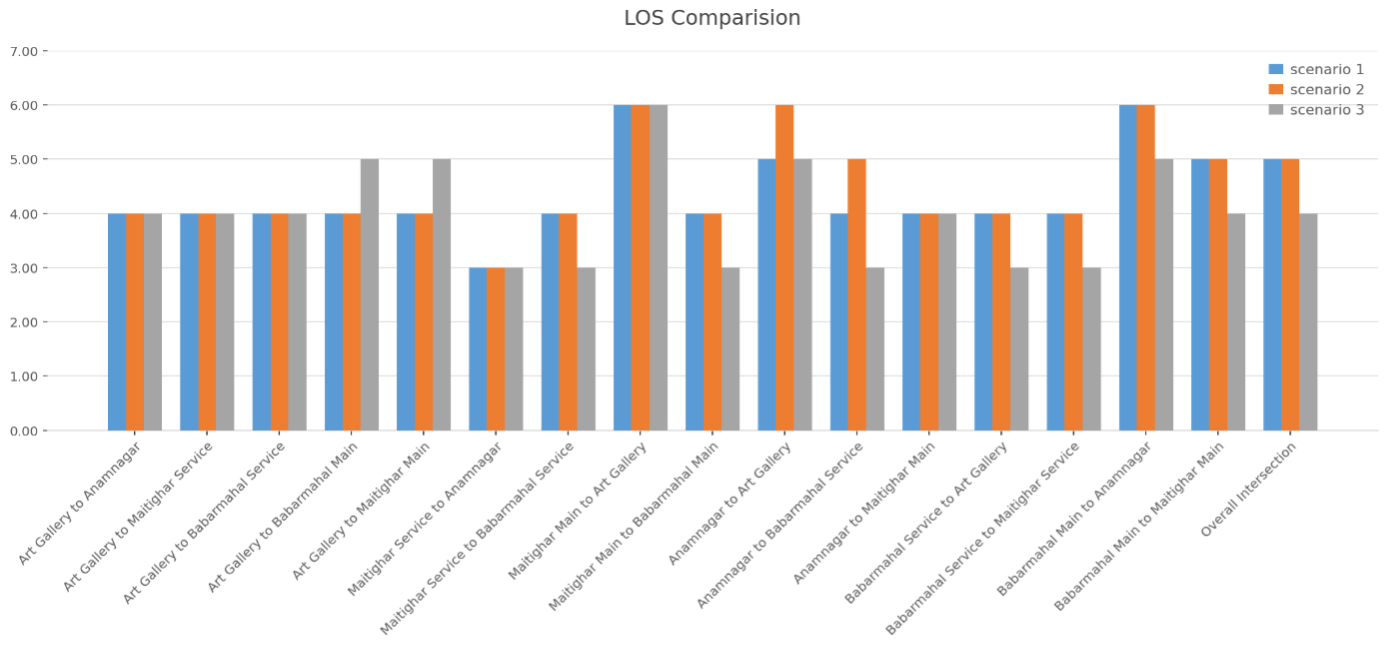
\includegraphics[width=\textwidth ]{src/images/figures/7.png}
    \caption{LOS: Peak Hour}
 \end{figure}


The off-peak hour LOS comparison across the three scenarios 
demonstrates that Scenario 3 consistently achieves the lowest 
or equal LOS values across nearly all movements, confirming 
its superiority as the most effective signal timing plan. 
The overall intersection LOS improves from 4 (Scenario 1) $\rightarrow$ 
4 (Scenario 2) $\rightarrow$ 4 (Scenario 3), indicating that 
while the overall grade remains unchanged during off-peak 
conditions, movement-level improvements are evident throughout. 
The most notable reductions are observed at Art Gallery to 
Maitighar Main and Maitighar Service to Babarmahal Service, 
where LOS drops from 5 under Scenarios 1 and 2 to 3 under 
Scenario 3, representing a two-grade improvement. The 
Maitighar Main to Art Gallery movement records the highest 
LOS of 6 across all three scenarios, indicating persistent 
congestion on this movement even during off-peak hours that 
could not be resolved through fixed-time signal optimization 
alone. For the majority of movements, including Art Gallery 
to Anamnagar, Art Gallery to Babarmahal Service, Art Gallery 
to Babarmahal Main, and Anamnagar-related movements, LOS 
remains at 4 across all scenarios, suggesting that off-peak 
traffic demand on these approaches is moderate and relatively 
insensitive to signal timing changes. Overall, Scenario 3 
delivers the most consistent and balanced LOS distribution 
across the intersection during off-peak conditions.


 \subsection{Off-Peak Hour Analysis}

 The figure displays the Level of Service (LOS) comparison 
 across three scenarios for various traffic routes and 
 intersections.
 
 \begin{figure}[ht]
    \centering
    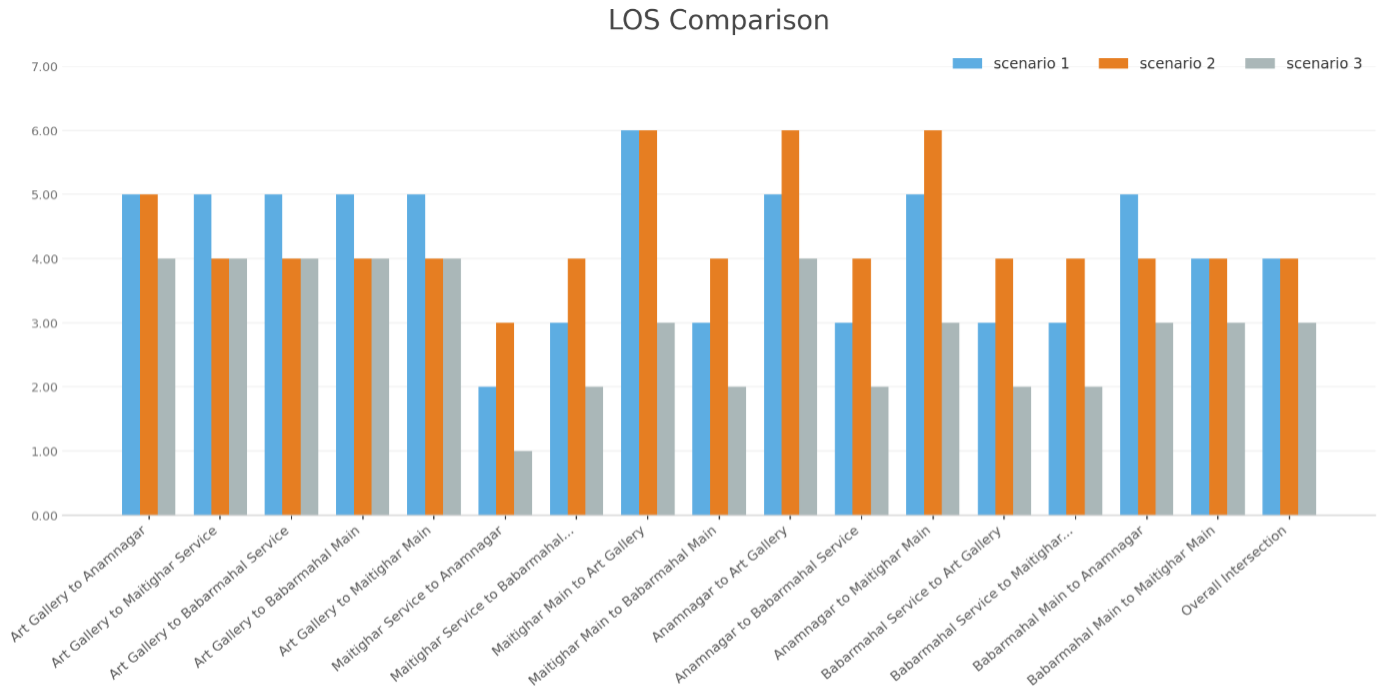
\includegraphics[width=\textwidth ]{src/images/figures/8.png}
    \caption{LOS: Off-Peak Hour}
 \end{figure}

 The most telling indicator is the overall intersection Level 
 of Service, which moves from 
 LOS D (S1) $\rightarrow$ LOS D (S2) $\rightarrow$ LOS 
 C (S3). This reveals that Scenario 2 produced no improvement 
 over the baseline, while Scenario 3 achieved a meaningful 
 upgrade by one service level, the most significant 
 system-wide improvement. 

 Maitighar Main to Art Gallery movement stands out as the 
 most striking improvement across all scenarios. Operating 
 at the worst possible service level of LOS F in Scenario 1, 
 it remained at LOS\_F in Scenario 2, indicating that early 
 interventions were entirely ineffective for this approach. 
 However, in Scenario 3, the Level of Service improved 
 dramatically to LOS C, a jump of three service levels from 
 the baseline, representing the most substantial LOS gain 
 recorded across the entire intersection. 

